\chapter{Numerics}
According to \cite{erlebacher1985finite} the Gaus divergenze theorem can be rewritten as
\begin{equation}
  \label{eqn:gauss}
  \int_V \nabla \vec{F} \,\, \mathrm{d}^n V = \oint_S \vec{F} \cdot \vec{n} \,\, \mathrm{d}^{n-1}S
\end{equation}
Using $\nabla f$ for $\vec{f}$ Eqn.~(\ref{eqn:gauss}) can be rewritten as
\begin{equation}
  \int_V \nabla^2 f \,\, \mathrm{d}^n V = \oint_S (\nabla f) \cdot \vec{n} \,\, \mathrm{d}^{n-1}S
\end{equation}
For the numerical solution a cell wise desrcitization is made.
Assuming that $\nabla^2 f$ is constants over a cell the equation above reduces to
\begin{equation}
  V_C \cdot \nabla^2 f = \sum_i^N (\nabla f) \cdot \vec{n}_i \cdot A_{i}.
\end{equation}

\section{2D Application for triangular mesh}
For a trinagular mesh assuming
%----------------------------------------------------------------
\begin{figure}[ht]
    \label{fig:rod_heat_transfer}
    \centering
    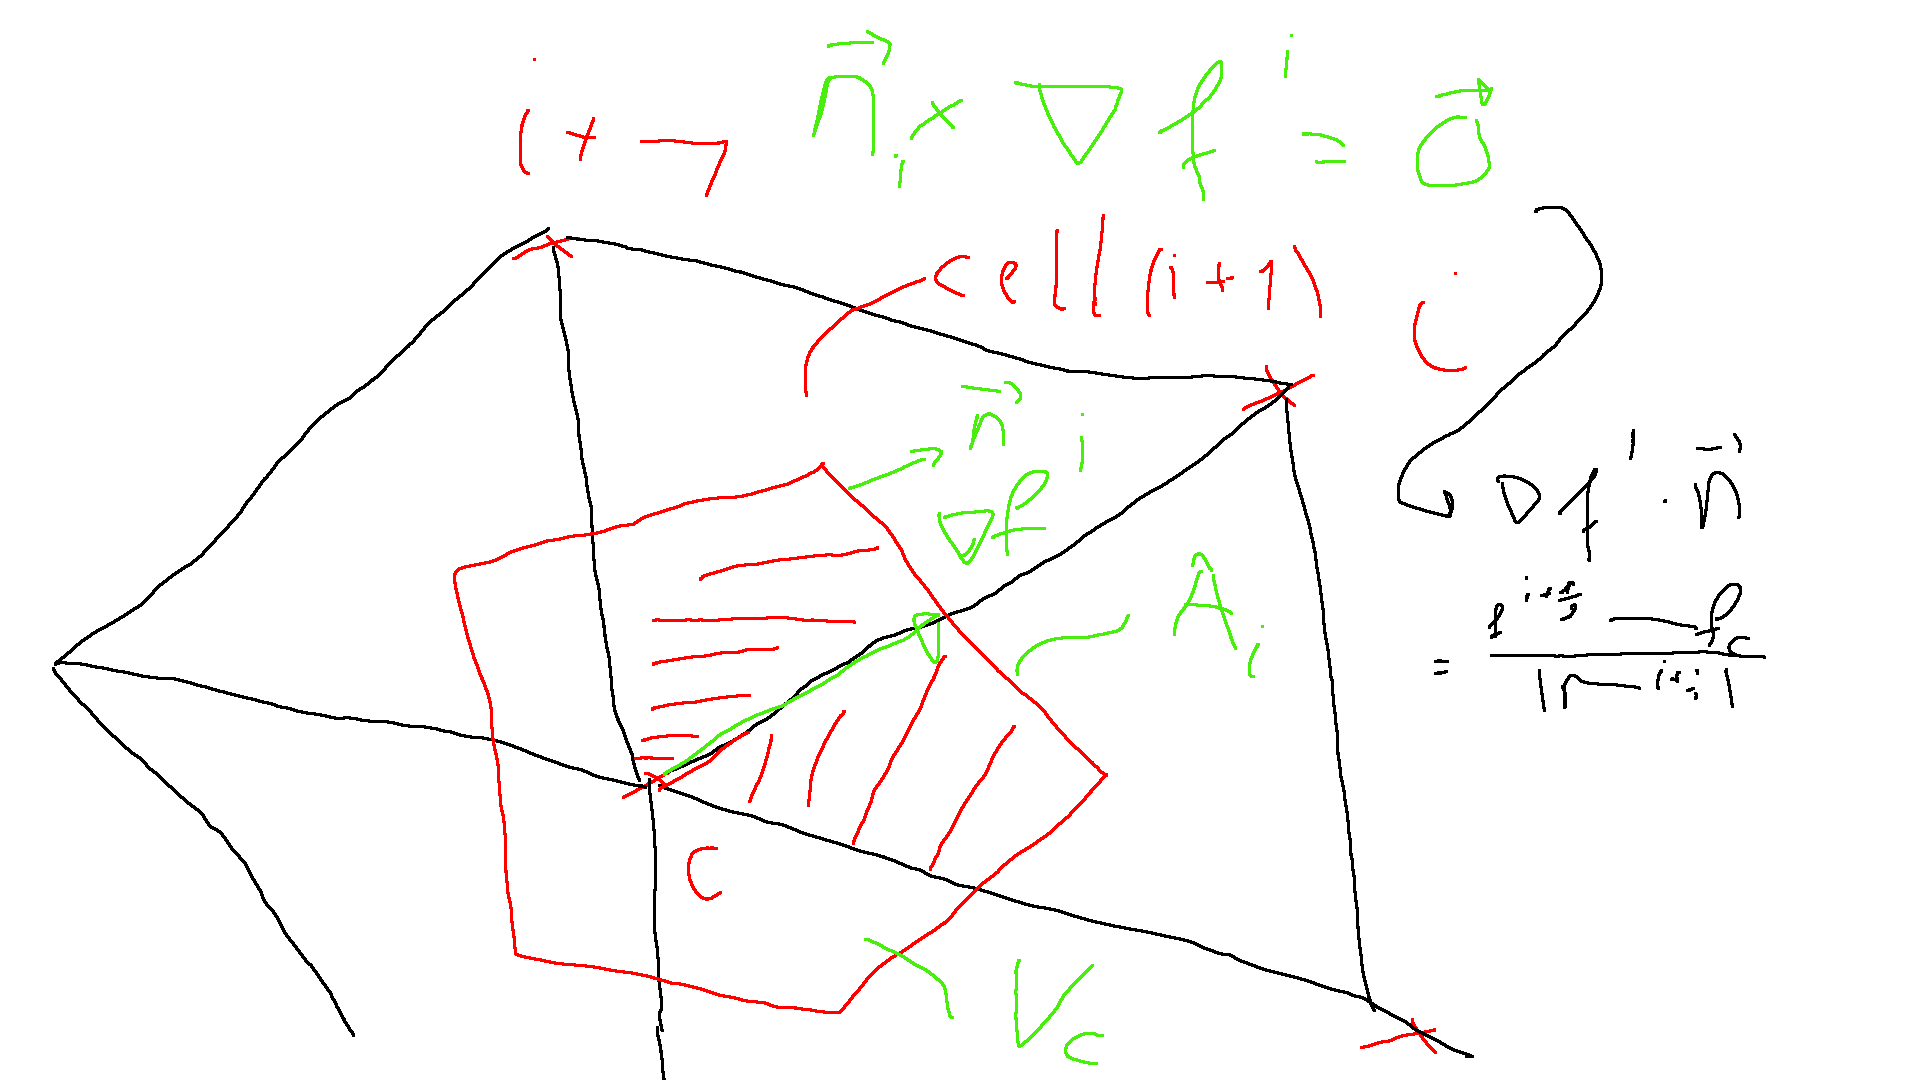
\includegraphics[width=0.8\linewidth]{draft.png}
    \caption{Test}
\end{figure}
%----------------------------------------------------------------
one can write
%----------------------------------------------------------------
\begin{equation}
  \nabla f \cdot \vec{n}_i = \frac{f_{i} - f_C}{|\vec{r}_{i}|}
\end{equation}
%----------------------------------------------------------------
for a 2d geometriy $A_{C, i}$ becomes a line segment
%----------------------------------------------------------------
\begin{equation}
  A_{i} = |\vec{b}_{i + 1} - \vec{b}_{i}| = L_i
\end{equation}
%----------------------------------------------------------------
where $\vec{b}_i$ is the barycentre of the last cell containing the point $i$.
In this context $V_C$ becomes the volume of created new cell $A_C$ which is defined as
%----------------------------------------------------------------
\begin{equation}
  A_C = \frac{1}{2} \cdot \sum_i^N  \vec{b}_{i + 1} \times \vec{b}_{i}
\end{equation}
%----------------------------------------------------------------
This leads to
%----------------------------------------------------------------
\begin{equation}
  \nabla^2 f = \frac{1}{A_C} \cdot \sum_i^N \frac{f_{i} - f_C}{|\vec{r}_{i}|} \cdot |\vec{b}_{i + 1} - \vec{b}_{i}| .
\end{equation}
%----------------------------------------------------------------

\section{Gradient}
Is given as
\begin{equation}
  \nabla f_c = \frac{1}{2 A_c} \sum_{i = 1}^3 f_i \cdot
  \begin{bmatrix}
    -e_{i, y} \\
    e_{i, x} \\
    e_{i, z}
  \end{bmatrix}
\end{equation}
where $\vec{e}_i$ is the vector reptreseting the ith vertex and is rotated to point to the cell centre and $f_i$ is the function value at the vertix i.
\begin{equation}
  f_i = \frac{1}{2} \cdot (f_{i, 0} + f_{i, 1})
\end{equation}
where $f_{i, k}$ is the value of the kth node of the vertex.
\begin{equation}
  \vec{e}_i = \vec{e}_{i, 1} - \vec{e}_{i, 0}
\end{equation}
Leads to
\begin{equation}
  \nabla f_c = \frac{1}{4 A_c} \sum_{k = 2}^3 \left( (f_k + f_{k - 1}) \cdot
  \begin{bmatrix}
    -(\vec{x}_{k} - \vec{x}_{k - 1})_y\\
    (\vec{x}_{k} - \vec{x}_{k - 1})_x \\
    (\vec{x}_{k} - \vec{x}_{k - 1})_z
  \end{bmatrix}
  \right)
\end{equation}
The derevative at given point $p$ sorounded by cells is given as
\begin{equation}
  \nabla f_p = \frac{1}{\sum_{c = 1}^N A_c} \cdot \sum_{c = 1}^N \nabla f_c \cdot A_c
\end{equation}
since we are only interested in the normal derivative at point p
\begin{equation}
  \left|\nabla f_p\right|_{\vec{n}_p} = \frac{1}{\sum_{c = 1}^N A_c} \cdot \sum_{c = 1}^N \nabla f_c \cdot \vec{n}_p \cdot A_c
\end{equation}

\section{Gradient 2}
Eqn.~(\ref{eqn:gauss})
\begin{equation}
  \int_V \vec{c} \cdot \nabla f \,\, \mathrm{d}^n V = \oint_S \vec{c} f \cdot \vec{n} \,\, \mathrm{d}^{n-1}S + \underbrace{\int_V f (\nabla \cdot \vec{c}) \,\, \mathrm{d}^n V}_{=0 \text{ for } \vec{c} = const}
\end{equation}
interpreting $\vec{c}$ as the normal of the wall at which the gradient is given ($\vec{n}_g$) leads to
\begin{equation}
  \int_V \nabla_{\vec{n}_g} f \,\, \mathrm{d}^n V = \oint_S f \cdot (\vec{n}_g  \cdot \vec{n}) \,\, \mathrm{d}^{n-1}S
\end{equation}
Discritezising over a cell and assuming const $\nabla_{\vec{n}_g} f$ over cell leads to
\begin{equation}
  A_c \cdot \nabla_{\vec{n}_g}f  = \sum_{i=1}^3 \frac{1}{2} \cdot (f_{i + 1} + f_i) \cdot (\vec{n}_g  \cdot \underbrace{\vec{n}_i \cdot S_i}_{M \cdot (\vec{x}_{i + 1} - \vec{x}_{i})})
\end{equation}
within\begin{equation}
  \vec{r}_{i+1, i} = \vec{x}_{i + 1} - \vec{x}_{i}
\end{equation}
and
\begin{equation}
  M =
  \begin{bmatrix}
    0 & 1 & 0 \\
    -1 & 0 & 0 \\
    0 & 0 & 1
  \end{bmatrix}
\end{equation}
is
\begin{equation}
  M \cdot \vec{r}_{i+1, i} =
  \begin{bmatrix}
    r_{i+1, i, y} \\
    -r_{i+1, i, x} \\
    r_{i+1, i, z}
  \end{bmatrix}
  = \vec{p}_{i+1, i}
\end{equation}
leads to
\begin{equation}
  \nabla_{\vec{n}_g}f  = \sum_{i=1}^2   \frac{f_{i + 1} + f_i}{2 A_c} \cdot \vec{n}_g  \cdot \vec{p}_{i+1, i} + \frac{f_1 + f_3}{2 A_c} \cdot \vec{n}_g  \cdot \vec{p}_{1, 3}
\end{equation}
